% Section 14: Abstract environments and selective sensing (key env)
% src: H5 (all) as repaired by critic V11, V12 and Sections 2.2, 2.3, 2.6, 2.7; H1 Section 6 (H1-R26, H1-R27) at its reading levels; H3-E2, H3-E3 by reference to sec:met
\section{Abstract environments and selective sensing}\label{sec:env}

The author's fifth idea gives meta-agents external states of their own: a corporation senses an informational environment of prices and indices rather than a physical medium, people sense the economy, and nerve cells sense chemical potentials but not gravity. \Cref{sec:met} declares a meta-agent's external states as linear functions of the joint process and asks when they have closed dynamics. This section treats, in linear-Gaussian exteriors, the prior question of part H5c of hypothesis H5 for an agent at any level, which functions of its exterior it should sense, by stating what a sensor optimal for a declared horizon-$h$ predictive-information objective reads (\cref{def:env-attention-objective}); the one-step expected free energy of the framework does not imply this objective and can oppose it (\cref{rem:env-efe-horizon-free,rem:env-two-step}). Sensors with a fixed number of channels or a Shannon budget that carry most information about the exterior at a horizon read the leading canonical variates between present and future (\cref{thm:env-canonical}); the horizon decides how many and which (\cref{prop:env-horizon,prop:env-diffusive}); preferences and control select within this order and can reverse it (\cref{thm:env-control,ex:env-fast-preference}). A selection principle of coupling, predictability and relevance (\cref{prop:env-selection}) turns the nerve cell into a model in which gravity fails the coupling clause by more than thirteen orders of magnitude per single-particle reading, and by nearly ten at equal pooling of molecular samples (\cref{ex:env-cell}). Aggregates of many agents are closed environments when the population consists of interchangeable types and carry memory otherwise (\cref{prop:env-aggregate-closure,prop:env-aggregate-memory}), and long-horizon decisions need few of them (\cref{thm:env-hayek-horizon,ex:env-firm,ex:env-person}). The main text states the sensor theorem, the dependence on the horizon, the control theorem and the Hayek dimension at a horizon; the lemma on summaries of the past, the diffusive case, the remarks on expected free energy, the selection principle with the cell model, the closure and memory of aggregates, the worked firm and person, sensing across levels and memberships, and the open problems are in the Supplement.

Theorems are for linear-Gaussian models. The exterior is a stationary Gauss--Markov process $\eta_{t+1}=F\eta_t+w_t$ with $\rho(F)<1$ and $Q\succ0$, so that every canonical correlation between $\eta_t$ and $\eta_{t+h}$ is below one; for the exterior's own dynamics this is the spectral contraction (C$_\rho$) with the stationary moment bound (M) of \cref{asm:sca-standing}, on which every correlation time below is conditional. Sensors are linear with Gaussian noise independent of everything else. The capacity of a sensor is either its number $\kappa$ of scalar channels, the attention capacity of \cref{def:fw-system} measured in channels, or its Shannon information $I(s;\eta_t)$ in nats, bounded by a budget $I_{\max}$. The horizon $h\ge1$ is a fixed number of rounds. For a matrix $X$, $\sigma_{\mathsf j}(X)$ is its $\mathsf j$-th largest singular value and $\lambda_{\mathsf j}(X)$ its $\mathsf j$-th eigenvalue, in decreasing order for symmetric matrices and by decreasing modulus otherwise. The $\mathsf u_{\mathsf j}$ are left eigenvectors of $F$, the mode amplitudes are $\mathsf u_{\mathsf j}^\top\eta$, and $\tau_{\mathsf j}=-1/\ln\lvert\lambda_{\mathsf j}(F)\rvert$ is the correlation time of mode $\mathsf j$.

\subsection{Linear sensors and canonical variates}\label{sec:env-sensors}

\begin{definition}[Linear sensors and canonical variates]\label{def:env-sensor}
Let $\mathsf X\in\R^{d_{\mathsf X}}$, what a sensor can read, and $\mathsf Y\in\R^{d_{\mathsf Y}}$, what is to be predicted, be jointly Gaussian with mean zero, covariances $\Sigma_{\mathsf X}\succ0$ and $\Sigma_{\mathsf Y}\succ0$ and cross-covariance $\Sigma_{\mathsf X\mathsf Y}$. The canonical correlations $1\ge\sigma_1\ge\sigma_2\ge\dots$ are the singular values of the whitened cross-covariance $\mathsf C=\Sigma_{\mathsf X}^{-1/2}\Sigma_{\mathsf X\mathsf Y}\Sigma_{\mathsf Y}^{-1/2}$, padded with zeros to length $d_{\mathsf X}$, and $\sigma_{\mathsf j}=0$ for $\mathsf j>d_{\mathsf X}$; with orthonormal left singular vectors $\mathsf e_{\mathsf j}$, the canonical variates $\mathsf e_{\mathsf j}^\top\Sigma_{\mathsf X}^{-1/2}\mathsf X$ are uncorrelated with unit variance \citep{hotelling1936relations}. A sensor with $\kappa$ channels is $s=H\mathsf X+v$, with $H\in\R^{\kappa\times d_{\mathsf X}}$ and $v\sim\Ncal(0,I_\kappa)$ independent of $(\mathsf X,\mathsf Y)$; a noise covariance $R\succ0$ reduces to this form by $s\mapsto R^{-1/2}s$. With the whitened sensor $\tilde H=H\Sigma_{\mathsf X}^{1/2}$, its captured covariance is
\[
\mathsf G_s=\tilde H^\top\bigl(I_\kappa+\tilde H\tilde H^\top\bigr)^{-1}\tilde H,
\]
whose eigenvalues $\mathsf g_1\ge\mathsf g_2\ge\dots$, the captured fractions, lie in $[0,1)$, at most $\kappa$ of them positive. When $\kappa>d_{\mathsf X}$ we put $\mathsf g_{\mathsf j}=0$ for $\mathsf j>d_{\mathsf X}$, and likewise $\lambda_{\mathsf j}(\mathsf J)=0$ for $\mathsf j>d_{\mathsf X}$ when $\mathsf J\succeq0$ is a symmetric $d_{\mathsf X}\times d_{\mathsf X}$ matrix, so that a channel beyond the $d_{\mathsf X}$-th carries noise only. The sensor reads the variate $f^\top\Sigma_{\mathsf X}^{-1/2}\mathsf X$ with captured fraction $\mathsf g>0$ when $\mathsf G_sf=\mathsf gf$ and $\lvert f\rvert=1$. A noiseless sensor $s=H\mathsf X$ of rank $\kappa$ has as captured covariance the orthogonal projector onto the row space of $\tilde H$.
\end{definition}
% src: H5-D1 (captured covariance renamed G_s, critic 2.7)

\begin{lemma}[Information and error of a linear sensor]\label{lem:env-information}
In the setting of \cref{def:env-sensor}:
\begin{enumerate}
\item[(i)] $\Cov(\Sigma_{\mathsf X}^{-1/2}\mathsf X\mid s)=I-\mathsf G_s$ and $I(s;\mathsf X)=-\frac12\sum_{\mathsf j}\ln(1-\mathsf g_{\mathsf j})$;
\item[(ii)] $I(s;\mathsf Y)=-\frac12\ln\det(I-\mathsf C^\top\mathsf G_s\mathsf C)$;
\item[(iii)] for every $\Upsilon\succeq0$, $\tr(\Upsilon\Cov(\mathsf Y\mid s))=\tr(\Upsilon\Sigma_{\mathsf Y})-\tr(\mathsf G_s\mathsf J_\Upsilon)$, with the decision matrix $\mathsf J_\Upsilon=\Sigma_{\mathsf X}^{-1/2}\Sigma_{\mathsf X\mathsf Y}\Upsilon\Sigma_{\mathsf Y\mathsf X}\Sigma_{\mathsf X}^{-1/2}$;
\item[(iv)] the captured covariances of $\kappa$-channel sensors are exactly the symmetric matrices $\mathsf G$ with $0\preceq\mathsf G\prec I$ and $\rank\mathsf G\le\kappa$.
\end{enumerate}
Information, conditional covariances and weighted errors therefore depend on a sensor only through its captured covariance.
\end{lemma}
% src: H5-L1

Proof in \cref{app:env}; checked in \cref{chk:env-sensors}. The proofs rest on the eigenvalue inequalities of \cref{lem:env-eigen}, stated and proved in full in \cref{app:env}.

\begin{theorem}[Optimal linear sensors read canonical variates]\label{thm:env-canonical}
Let $(\mathsf X,\mathsf Y)$ be as in \cref{def:env-sensor} with $\sigma_1<1$, and let $s$ have $\kappa$ channels and captured fractions $\mathsf g_1\ge\dots\ge\mathsf g_\kappa$.
\begin{enumerate}
\item[(a)] (Information.) $I(s;\mathsf Y)\le-\frac12\sum_{\mathsf j\le\kappa}\ln(1-\mathsf g_{\mathsf j}\sigma_{\mathsf j}^2)$, with equality for the sensor whose $\mathsf j$-th channel reads the $\mathsf j$-th canonical variate, $s_{\mathsf j}=(\mathsf g_{\mathsf j}/(1-\mathsf g_{\mathsf j}))^{1/2}\mathsf e_{\mathsf j}^\top\Sigma_{\mathsf X}^{-1/2}\mathsf X+v_{\mathsf j}$.
\item[(b)] (Budget.) If $\sigma_1>0$ and $I_{\max}>0$, then
\[
\max\bigl\{I(s;\mathsf Y):I(s;\mathsf X)\le I_{\max}\bigr\}=\sum_{\substack{\mathsf j\le\kappa\\\sigma_{\mathsf j}^2>\mathsf v}}\frac12\ln\frac{1-\mathsf v}{1-\sigma_{\mathsf j}^2},
\]
where the water level $\mathsf v\in(0,\sigma_1^2)$ is the unique solution of $\sum_{\mathsf j\le\kappa,\sigma_{\mathsf j}^2>\mathsf v}\frac12\ln\frac{\sigma_{\mathsf j}^2(1-\mathsf v)}{\mathsf v(1-\sigma_{\mathsf j}^2)}=I_{\max}$. The maximum is attained by reading the canonical variates with $\sigma_{\mathsf j}^2>\mathsf v$, $\mathsf j\le\kappa$, with captured fractions $\mathsf g_{\mathsf j}=(\sigma_{\mathsf j}^2-\mathsf v)/(\sigma_{\mathsf j}^2(1-\mathsf v))$. The variates enter in the order of their canonical correlations as the budget grows, the $\mathsf m$-th when $I_{\max}$ exceeds $\mathcal I_{\mathsf m}=\sum_{\mathsf j<\mathsf m}\frac12\ln\frac{\sigma_{\mathsf j}^2(1-\sigma_{\mathsf m}^2)}{\sigma_{\mathsf m}^2(1-\sigma_{\mathsf j}^2)}$, with $\mathcal I_{\mathsf m}=+\infty$ when $\sigma_{\mathsf m}=0$. If $\sigma_1=0$ or $I_{\max}=0$ the maximum is $0$.
\item[(c)] (Weighted error.) For every symmetric $\mathsf J\succeq0$, $\tr(\mathsf G_s\mathsf J)\le\sum_{\mathsf j\le\kappa}\mathsf g_{\mathsf j}\lambda_{\mathsf j}(\mathsf J)$, with equality for the sensor that reads the leading eigenvectors of $\mathsf J$ in order. Under $I(s;\mathsf X)\le I_{\max}$ the largest value of $\tr(\mathsf G_s\mathsf J)$ is $0$ if $\mathsf J=0$ or $I_{\max}=0$, and otherwise $\sum_{\mathsf j\le\kappa}(\lambda_{\mathsf j}(\mathsf J)-\mathsf v')^+$, attained with $\mathsf g_{\mathsf j}=(1-\mathsf v'/\lambda_{\mathsf j}(\mathsf J))^+$ for $\lambda_{\mathsf j}(\mathsf J)>0$ and $\mathsf g_{\mathsf j}=0$ otherwise, with $\mathsf v'\in(0,\lambda_1(\mathsf J))$ the unique solution of $\sum_{\mathsf j\le\kappa}\frac12\ln^+(\lambda_{\mathsf j}(\mathsf J)/\mathsf v')=I_{\max}$. With $\mathsf J=\mathsf J_\Upsilon$ this minimizes the weighted error of \cref{lem:env-information}(iii).
\item[(d)] (When the criteria agree.) For $\Upsilon=\Sigma_{\mathsf Y}^{-1}$, $\mathsf J_\Upsilon=\mathsf C\mathsf C^\top$, whose eigenvectors are the $\mathsf e_{\mathsf j}$ with eigenvalues $\sigma_{\mathsf j}^2$: both criteria read leading canonical variates, and at equal budget the information criterion reads no more of them than the error criterion. For other weights the error criterion reads leading eigenvectors of $\mathsf J_\Upsilon$, which need not be the leading canonical variates (\cref{prop:env-horizon}(c)); when $\mathsf J_\Upsilon$ and $\mathsf C\mathsf C^\top$ do not commute, no orthonormal eigenbasis of $\mathsf J_\Upsilon$ consists of left singular vectors of $\mathsf C$, so the eigenvectors of $\mathsf J_\Upsilon$ are not all canonical variates.
\item[(e)] (Noiseless sensors.) If $\rank H=\kappa$, then $I(H\mathsf X;\mathsf Y)\le-\frac12\sum_{\mathsf j\le\kappa}\ln(1-\sigma_{\mathsf j}^2)$, and if $\sigma_\kappa>\sigma_{\kappa+1}$ equality holds exactly when the row space of $H\Sigma_{\mathsf X}^{1/2}$ is spanned by $\mathsf e_1,\dots,\mathsf e_\kappa$. Likewise $\tr(\Upsilon\Cov(\mathsf Y\mid H\mathsf X))\ge\tr(\Upsilon\Sigma_{\mathsf Y})-\sum_{\mathsf j\le\kappa}\lambda_{\mathsf j}(\mathsf J_\Upsilon)$, with equality for the top-$\kappa$ eigenspace of $\mathsf J_\Upsilon$.
\end{enumerate}
\end{theorem}
% src: H5-T1; critic V11 (attribution of (b) and (c); novelty restricted)

Proof in \cref{app:env}; checked in \cref{chk:env-sensors}. In (b), when $\sigma_1=0$ the matrix $\mathsf C$ vanishes and $I(s;\mathsf Y)=0$ for every sensor by \cref{lem:env-information}(ii), and when $I_{\max}=0$, \cref{lem:env-information}(i) forces $\mathsf G_s=0$; the value is $0$ in both cases. In (c), when $\mathsf J\neq0$ the left side of the equation for $\mathsf v'$ decreases continuously and strictly from $+\infty$ to $0$ on $(0,\lambda_1(\mathsf J)]$, which gives the water level when $I_{\max}>0$; when $\mathsf J=0$, $\tr(\mathsf G_s\mathsf J)=0$ for every sensor and, for $I_{\max}>0$, the equation has no positive solution; and when $I_{\max}=0$, \cref{lem:env-information}(i) forces $\mathsf G_s=0$. Part (b) has the form of water-filling over parallel Gaussian channels, capacity going to the variates above a common level, and part (c) is reverse water-filling, the Gaussian rate-distortion solution; both classical solutions are in \citet{cover2006elements}, and the proof reduces the sensor problem to separable allocations of these forms through \cref{lem:env-information}. The Lagrangian form of (b), minimizing $I(s;\mathsf X)-\mathsf tI(s;\mathsf Y)$ over noisy linear projections without a rank limit, is the Gaussian information bottleneck, whose optimal projection Theorem~3.1 of \citet{chechik2005information} builds from the eigenvectors of $\Sigma_{\mathsf X\mid\mathsf Y}\Sigma_{\mathsf X}^{-1}$, each entering at the critical value $1/(1-\mathsf l)$ of the trade-off parameter $\mathsf t$ for its eigenvalue $\mathsf l$. These eigenvalues are $1-\sigma_{\mathsf j}^2$, so the critical values are $\sigma_{\mathsf j}^{-2}$, which is the condition $\sigma_{\mathsf j}^2>\mathsf v$ with $\mathsf v=1/\mathsf t$. The budget form is in the same paper: its Section~5 gives in closed form the information curve, the largest $I(s;\mathsf Y)$ as a function of $I(s;\mathsf X)$, and shows that it is concave, and its Section~8 describes the solution as the best linear projection under a constraint on $I(s;\mathsf X)$ and names a dimension fixed in advance as the alternative way to limit the projection. What (b) adds to that paper is therefore at most the joint treatment of the cap $\kappa$ on the number of channels and the budget. Rank reduction and a rate budget in canonical coordinates are treated together by \citet{scharf1998wiener}, whose Section~V discards the measurement coordinates of small squared canonical correlation and allocates a bit budget over the remaining ones so as to minimize the trace of the error covariance, a single slicing level fixing the rank, the allocation and the distortion. Part (c) has this form for a general weight, with the rank limit imposed separately from the budget, and part (b) is its counterpart for predictive information; we claim no priority for either. The linear past-future bottleneck \citep{creutzig2009past}, which we know from its abstract, is a further precedent for (b) that we have not compared with it in detail. We do not claim that linear-Gaussian sensors are optimal among all sensors.

For a fully observed stationary Gauss--Markov exterior a summary of the past, under the same limits on dimension and information, carries no more information about the exterior at the horizon, or about a selected part of it, than the optimal sensor of the present state (Supplement, \cref{lem:env-markov}, under the hypotheses stated there), so the sensor problem is posed on the pair $(\eta_t,\eta_{t+h})$, with $\Sigma_{\mathsf X}=P_0$ the stationary covariance.

\subsection{How the selection depends on the horizon}\label{sec:env-horizon}

For $\mathsf X=\eta_t$ and $\mathsf Y=\eta_{t+h}$ the whitened cross-covariance is $\mathsf C(h)=P_0^{1/2}(F^h)^\top P_0^{-1/2}=(\mathsf F^h)^\top$, with the whitened transition $\mathsf F=P_0^{-1/2}FP_0^{1/2}$.

\begin{proposition}[Horizon dependence]\label{prop:env-horizon}
Let $\mathsf X=\eta_t$ and $\mathsf Y=\eta_{t+h}$.
\begin{enumerate}
\item[(a)] (Reversible exteriors.) If $FP_0=P_0F^\top$, then $\mathsf F$ is symmetric, the canonical correlations are $\sigma_{\mathsf j}(h)=\lvert\lambda_{\mathsf j}(F)\rvert^h=e^{-h/\tau_{\mathsf j}}$, and the canonical variates are the mode amplitudes $\mathsf u_{\mathsf j}^\top\eta_t$, normalized by $\mathsf u_{\mathsf j}^\top P_0\mathsf u_{\mathsf j}=1$, the same at every horizon. The noiseless rank-$\kappa$ optimum reads the $\kappa$ slowest modes at every $h$, and the information it captures, $-\frac12\sum_{\mathsf j\le\kappa}\ln(1-e^{-2h/\tau_{\mathsf j}})$, decreases with $h$. If the moduli are distinct, under the budget $I_{\max}$ mode $\mathsf m\le\kappa$ is read exactly when $I_{\max}>\mathcal I_{\mathsf m}(h)$, the threshold of \cref{thm:env-canonical}(b); each $\mathcal I_{\mathsf m}(h)$ is non-decreasing in $h$ with $\mathcal I_{\mathsf m}(h)\ge h\sum_{\mathsf j<\mathsf m}(\tau_{\mathsf m}^{-1}-\tau_{\mathsf j}^{-1})$, so the number of modes read is non-increasing in $h$, and only the slowest mode is read once $h>I_{\max}/(\tau_2^{-1}-\tau_1^{-1})$.
\item[(b)] (Non-reversible exteriors.) Let $F$ be diagonalizable with $\lvert\lambda_\kappa(F)\rvert>\lvert\lambda_{\kappa+1}(F)\rvert$, let $\mathbb P_{\mathrm{slow}}$ be its real spectral projector on the $\kappa$ eigenvalues of largest modulus, $\mathcal U_\kappa$ the real span of the corresponding $\mathsf u_{\mathsf j}$, and $\vartheta_h$ the largest principal angle between a top-$\kappa$ canonical subspace, in whitened coordinates, and $P_0^{1/2}\mathcal U_\kappa$. With $\mathsf c_P=\Vert P_0^{1/2}\Vert\Vert P_0^{-1/2}\Vert$, $\mathfrak a_h=\mathsf c_P\Vert F^h(I-\mathbb P_{\mathrm{slow}})\Vert$ and $\mathfrak b_h=\sigma_\kappa(F^h\mathbb P_{\mathrm{slow}})/\mathsf c_P$,
\[
\sin\vartheta_h\le\frac{\mathfrak a_h}{\mathfrak b_h-\mathfrak a_h}\qquad\text{whenever }\mathfrak a_h<\mathfrak b_h,
\]
and $\mathfrak a_h/\mathfrak b_h=O\bigl((\lvert\lambda_{\kappa+1}(F)\rvert/\lvert\lambda_\kappa(F)\rvert)^h\bigr)$, with the eigenvector constants of \eqref{eq:env-ab-bounds} in \cref{app:env}. Hence $\sin\vartheta_h=O\bigl((\lvert\lambda_{\kappa+1}(F)\rvert/\lvert\lambda_\kappa(F)\rvert)^h\bigr)$ as $h\to\infty$: the sensors of the long-horizon optimum read the slow mode amplitudes. The same holds for the error criterion with weight $\Upsilon$, with $F^h$ replaced by $\Upsilon^{1/2}F^h$, when $\Upsilon^{1/2}F^h\mathbb P_{\mathrm{slow}}$ has rank $\kappa$.
\item[(c)] (Fixed error weights.) Let $F$ be symmetric with $QF=FQ$, with modes of eigenvalues $\lambda_{\mathsf j}(F)$ and stationary variances $\mathsf p_{\mathsf j}=\lambda_{\mathsf j}(Q)/(1-\lambda_{\mathsf j}(F)^2)$ in a common eigenbasis, and $\Upsilon=I$. The rank-one error optimum reads the mode that maximizes $\lambda_{\mathsf j}(F)^{2h}\mathsf p_{\mathsf j}$. For a slow mode $\mathrm s$ and a fast mode $\mathrm f$ with $\lvert\lambda_{\mathrm s}(F)\rvert>\lvert\lambda_{\mathrm f}(F)\rvert$ and $\mathsf p_{\mathrm f}>\mathsf p_{\mathrm s}$, the error criterion ranks the fast mode above the slow mode for $h<h^\ast$ and below it for $h>h^\ast$, with $h^\ast=\ln(\mathsf p_{\mathrm f}/\mathsf p_{\mathrm s})/(2\ln(\lvert\lambda_{\mathrm s}(F)\rvert/\lvert\lambda_{\mathrm f}(F)\rvert))$, while the information criterion ranks the slow mode above the fast mode at every $h\ge1$. If $\mathrm s$ and $\mathrm f$ are the only two modes, the rank-one error optimum therefore reads the fast mode for $h<h^\ast$ and the slow mode for $h>h^\ast$, while the information criterion reads the slow mode at every $h\ge1$; with further modes either criterion can read a third mode.
\end{enumerate}
\end{proposition}
% src: H5-P1; critic V11 ((b) stated with its constant and as an asymptotic statement)

Proof in \cref{app:env}; checked in \cref{chk:env-horizon}. The explicit bound in (b) is informative only at long horizons: in a computed non-normal instance its condition $\mathfrak a_h<\mathfrak b_h$ fails at every computed horizon up to 20 for $\kappa=1$, so that it bounds nothing there, while the angle itself decays at the geometric rate. \Citet{sachdeva2021optimal} report a rotation of this kind for a stochastically driven damped oscillator, whose optimal predictive representation turns as the prediction lag grows. In reversible exteriors, by contrast, the ranking stays fixed and only the number of variables read can change with $h$, without increasing. At one step the selection of slow features by a predictive-information criterion has a precedent in \citet{creutzig2008predictive}, whose abstract, which is what we read, states that linear slow feature analysis is a variant of predictive coding that maximizes the mutual information between the current output and the input at the next time step, in an information-bottleneck formulation; what (a) adds to it is at most the horizon $h$ and the budget thresholds, and we have not compared the two statements in detail. Part (c) shows that a prediction error with a weight other than $\Sigma_{\mathsf Y}^{-1}$ need not select the leading canonical variate (\cref{thm:env-canonical}(d)). \Cref{fig:env-horizon} draws the budgets $\mathcal I_{\mathsf m}(h)$ at which the variates of the four-mode exterior of \cref{chk:env-horizon}(a) enter: all three rise with the horizon, and at $I_{\max}=1.5$ nats the second variate is read only up to $h=12$, below the sufficient horizon $17.61$ of \cref{prop:env-horizon}(a).

\begin{figure}[t]
  \centering
  % Figure: activation budgets of a reversible exterior against the horizon (thm:env-canonical(b), prop:env-horizon(a)).
% Exterior of chk:env-horizon(a): four modes with lambda(F) = (0.98, 0.9, 0.7, 0.4) in an orthonormal basis, Q = 0.5 I,
% kappa = 4 channels (no rank limit), so sigma_j(h) = |lambda_j(F)|^h = exp(-h/tau_j) with tau_j^{-1} = -ln|lambda_j(F)|
% = 0.020203, 0.105361, 0.356675, 0.916291. Solid: I_k(h) = sum_{j<k} (1/2) ln[sigma_j^2 (1 - sigma_k^2) /
% (sigma_k^2 (1 - sigma_j^2))], the budget above which variate k is read (thm:env-canonical(b)), for k = 2, 3, 4 on
% 24 points per decade of real h in [1, 100] plus the check horizons. Dashed: the linear lower bound
% h sum_{j<k} (tau_k^{-1} - tau_j^{-1}) of prop:env-horizon(a), slopes 0.085158, 0.58779, 2.26663; the gap
% I_2 - bound is 0.784, 0.486, 0.0089 at h = 1, 10, 100. Recomputed in double precision: the singular values of the
% whitened cross-covariance P0^{-1/2} P0 (F^h)^T P0^{-1/2} of a random orthonormal realization (detailed balance to
% 9e-16) equal |lambda(F)|^h to 4e-8 relative for all four at h <= 20, and the I_2, I_3 they give at h = 40, 80 equal
% the closed form to four decimals (sigma_4 is below double-precision resolution there); water-filling with the
% water level found by bisection reads k - 1 variates just below I_k(h) and k just above it. Dots: I_2 = 0.8693,
% 0.9145, 1.0607, 1.3375, 1.9907, 3.5169, 6.8328 at h = 1, 2, 5, 10, 20, 40, 80, the values printed in
% chk:env-horizon(a). Dotted: fixed budgets of 1.5, 3 and 6 nats. At 1.5 nats I_2(h) = 1.5 at h = 12.664 (two
% variates for h <= 12, one from h = 13) and the bound reaches 1.5 at the sufficient horizon
% 1.5/(tau_2^{-1} - tau_1^{-1}) = 17.614 (circles). At 3 nats the count falls 3, 2, 1 at h = 2.746, 33.477; at 6 nats
% it falls 4, 3, 2, 1 at h = 1.748, 9.069, 70.101. I_3(1) = 2.3593 > 1.5, so a third variate is never read at 1.5 nats.
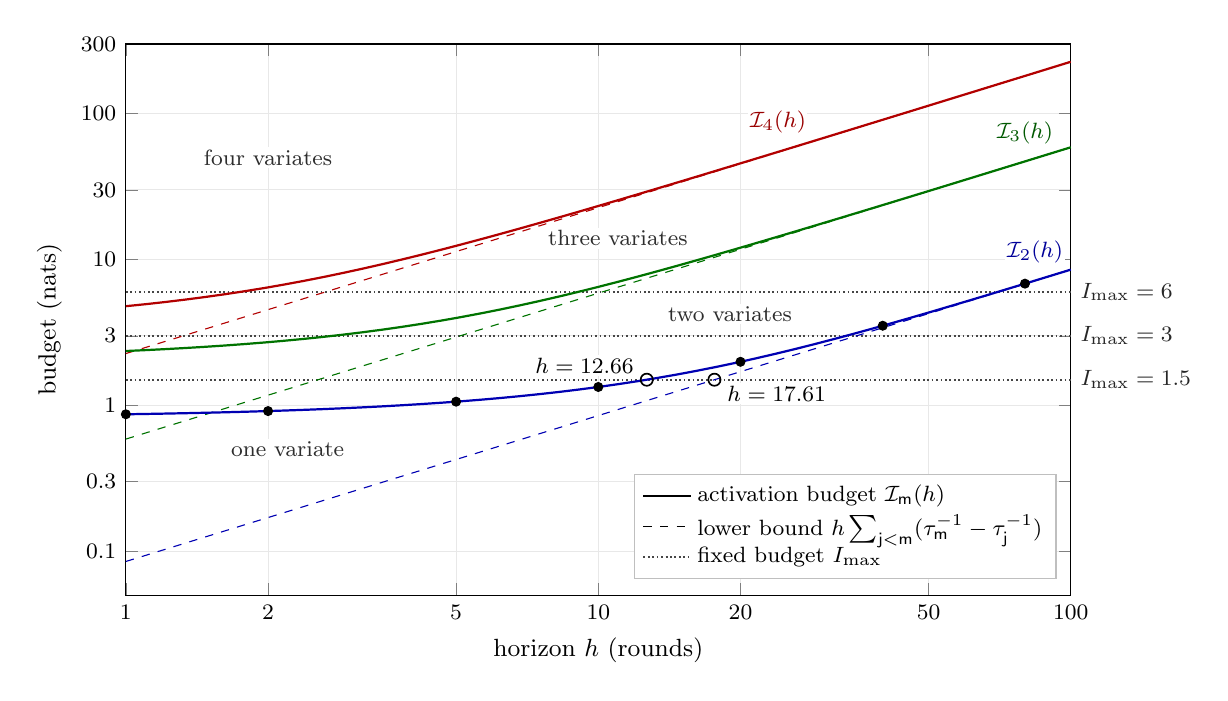
\begin{tikzpicture}
  \begin{axis}[width=12.0cm, height=7cm, scale only axis, xmode=log, ymode=log,
      xmin=1, xmax=100, ymin=0.05, ymax=300,
      xtick={1,2,5,10,20,50,100}, ytick={0.1,0.3,1,3,10,30,100,300}, log ticks with fixed point,
      grid=major, grid style={gray!18}, clip=false,
      xlabel={horizon $h$ (rounds)}, ylabel={budget (nats)},
      every axis label/.style={font=\small}, tick label style={font=\footnotesize},
      legend style={font=\footnotesize, at={(0.985,0.03)}, anchor=south east, draw=gray!50, fill=white,
        cells={anchor=west}, row sep=-1pt}]
    % fixed budgets
    \draw[gray!55!black, densely dotted, semithick] (axis cs:1,1.5) -- (axis cs:100,1.5);
    \draw[gray!55!black, densely dotted, semithick] (axis cs:1,3) -- (axis cs:100,3);
    \draw[gray!55!black, densely dotted, semithick] (axis cs:1,6) -- (axis cs:100,6);
    % linear lower bounds of prop:env-horizon(a), straight lines on these axes
    \addplot[blue!70!black, dashed, forget plot] coordinates {(1,0.085158) (100,8.5158)};
    \addplot[green!45!black, dashed, forget plot] coordinates {(1,0.58779) (100,58.779)};
    \addplot[red!70!black, dashed, forget plot] coordinates {(1,2.2666) (100,226.66)};
    % activation budgets I_2, I_3, I_4
    \addplot[blue!70!black, thick, forget plot] coordinates {(1,0.86926) (1.1007,0.87373) (1.2115,0.87868) (1.3335,0.88415) (1.4678,0.8902) (1.6156,0.8969) (1.7783,0.90432) (1.9573,0.91254) (2,0.9145) (2.1544,0.92165) (2.3714,0.93176) (2.6102,0.94298) (2.873,0.95545) (3.1623,0.96931) (3.4807,0.98474) (3.8312,1.0019) (4.217,1.0211) (4.6416,1.0425) (5,1.0607) (5.109,1.0663) (5.6234,1.0931) (6.1897,1.123) (6.8129,1.1565) (7.4989,1.1942) (8.254,1.2364) (9.0852,1.284) (10,1.3375) (11.007,1.3978) (12.115,1.4657) (13.335,1.5424) (14.678,1.6289) (16.156,1.7265) (17.783,1.8366) (19.573,1.9607) (20,1.9907) (21.544,2.1006) (23.714,2.2579) (26.102,2.4348) (28.73,2.6333) (31.623,2.8556) (34.807,3.1043) (38.312,3.382) (40,3.5169) (42.17,3.6914) (46.416,4.0358) (51.09,4.4185) (56.234,4.8432) (61.897,5.3138) (68.129,5.8347) (74.989,6.4107) (80,6.8328) (82.54,7.0471) (90.852,7.7496) (100,8.5247)};
    \addplot[green!45!black, thick, forget plot] coordinates {(1,2.3593) (1.1007,2.3931) (1.2115,2.4308) (1.3335,2.4729) (1.4678,2.5198) (1.6156,2.5723) (1.7783,2.631) (1.9573,2.6968) (2,2.7126) (2.1544,2.7705) (2.3714,2.8533) (2.6102,2.9463) (2.873,3.0509) (3.1623,3.1687) (3.4807,3.3014) (3.8312,3.451) (4.217,3.6197) (4.6416,3.81) (5,3.974) (5.109,4.0245) (5.6234,4.2662) (6.1897,4.5385) (6.8129,4.8449) (7.4989,5.1892) (8.254,5.5755) (9.0852,6.0084) (10,6.4926) (11.007,7.0333) (12.115,7.6361) (13.335,8.3071) (14.678,9.0529) (16.156,9.8808) (17.783,10.799) (19.573,11.815) (20,12.058) (21.544,12.94) (23.714,14.184) (26.102,15.558) (28.73,17.076) (31.623,18.751) (34.807,20.6) (38.312,22.639) (40,23.622) (42.17,24.887) (46.416,27.366) (51.09,30.098) (56.234,33.108) (61.897,36.425) (68.129,40.078) (74.989,44.103) (80,47.043) (82.54,48.534) (90.852,53.414) (100,58.788)};
    \addplot[red!70!black, thick, forget plot] coordinates {(1,4.7866) (1.1007,4.9402) (1.2115,5.113) (1.3335,5.3076) (1.4678,5.527) (1.6156,5.7742) (1.7783,6.053) (1.9573,6.3673) (2,6.4432) (2.1544,6.7215) (2.3714,7.1203) (2.6102,7.569) (2.873,8.0733) (3.1623,8.6392) (3.4807,9.2732) (3.8312,9.9825) (4.217,10.775) (4.6416,11.658) (5,12.411) (5.109,12.641) (5.6234,13.734) (6.1897,14.948) (6.8129,16.294) (7.4989,17.786) (8.254,19.437) (9.0852,21.263) (10,23.282) (11.007,25.513) (12.115,27.976) (13.335,30.695) (14.678,33.695) (16.156,37.004) (17.783,40.653) (19.573,44.676) (20,45.635) (21.544,49.11) (23.714,53.996) (26.102,59.379) (28.73,65.309) (31.623,71.841) (34.807,79.036) (38.312,86.959) (40,90.776) (42.17,95.684) (46.416,105.29) (51.09,115.87) (56.234,127.52) (61.897,140.34) (68.129,154.46) (74.989,170) (80,181.35) (82.54,187.11) (90.852,205.94) (100,226.67)};
    % values of chk:env-horizon(a) on I_2
    \addplot[only marks, mark=*, mark size=1.6pt, black, forget plot] coordinates {(1,0.8693) (2,0.9145) (5,1.0607) (10,1.3375) (20,1.9907) (40,3.5169) (80,6.8328)};
    % budget 1.5: I_2 reaches it at h = 12.664, the bound at the sufficient horizon 17.614
    \addplot[only marks, mark=o, mark size=2.2pt, black, semithick, forget plot] coordinates {(12.664,1.5) (17.614,1.5)};
    \node[font=\footnotesize, anchor=south east, inner sep=1pt, fill=white, xshift=-3.5pt, yshift=1pt] at (axis cs:12.664,1.5) {$h=12.66$};
    \node[font=\footnotesize, anchor=north west, inner sep=1pt, fill=white, xshift=3.5pt, yshift=-1pt] at (axis cs:17.614,1.5) {$h=17.61$};
    % curve labels
    \node[font=\footnotesize, blue!60!black, inner sep=0.5pt, fill=white] at (axis cs:84,11.2) {$\mathcal I_2(h)$};
    \node[font=\footnotesize, green!35!black, inner sep=0.5pt, fill=white] at (axis cs:80,74) {$\mathcal I_3(h)$};
    \node[font=\footnotesize, red!60!black, inner sep=0.5pt, fill=white] at (axis cs:24,88) {$\mathcal I_4(h)$};
    % regions: number of variates read at a budget in the region
    \node[font=\footnotesize, gray!35!black, inner sep=1pt, fill=white] at (axis cs:2.2,0.5) {one variate};
    \node[font=\footnotesize, gray!35!black, inner sep=1pt, fill=white] at (axis cs:19,4.24) {two variates};
    \node[font=\footnotesize, gray!35!black, inner sep=1pt, fill=white] at (axis cs:11,14) {three variates};
    \node[font=\footnotesize, gray!35!black, inner sep=1pt, fill=white] at (axis cs:2,50) {four variates};
    % budget labels outside the frame
    \node[font=\footnotesize, gray!30!black, anchor=west] at (axis cs:100,1.5) {$I_{\max}=1.5$};
    \node[font=\footnotesize, gray!30!black, anchor=west] at (axis cs:100,3) {$I_{\max}=3$};
    \node[font=\footnotesize, gray!30!black, anchor=west] at (axis cs:100,6) {$I_{\max}=6$};
    % legend of line styles
    \addlegendimage{black, thick}
    \addlegendentry{activation budget $\mathcal I_{\mathsf m}(h)$}
    \addlegendimage{black, dashed}
    \addlegendentry{lower bound $h\sum_{\mathsf j<\mathsf m}(\tau_{\mathsf m}^{-1}-\tau_{\mathsf j}^{-1})$}
    \addlegendimage{gray!55!black, densely dotted, semithick}
    \addlegendentry{fixed budget $I_{\max}$}
  \end{axis}
\end{tikzpicture}

  \caption{\textbf{Activation budgets rise with the horizon.} The budget $\mathcal I_{\mathsf m}(h)$ above which the $\mathsf m$-th canonical variate is read (\cref{thm:env-canonical}(b)), for $\mathsf m=2,3,4$ in the reversible exterior of \cref{chk:env-horizon}(a), with $\lambda(F)=(0.98,0.9,0.7,0.4)$, canonical correlations $\sigma_{\mathsf j}(h)=\lvert\lambda_{\mathsf j}(F)\rvert^h$ and $\kappa=4$ channels. The curves divide the plane into regions in which one to four variates are read. Each $\mathcal I_{\mathsf m}(h)$ is non-decreasing in $h$ and approaches its linear lower bound of \cref{prop:env-horizon}(a) (dashed) at long horizons, so the number of variates read at a fixed budget (dotted) falls as the horizon grows. With $I_{\max}=1.5$ nats two variates are read up to $h=12$ and one from $h=13$ on: $\mathcal I_2(h)$ reaches the budget at $h=12.66$, before the sufficient horizon $I_{\max}/(\tau_2^{-1}-\tau_1^{-1})=17.61$ at which its lower bound reaches it (circles). With $3$ nats the number falls from three to two and to one at $h=2.75$ and $33.48$, and with $6$ nats from four to three, two and one at $h=1.75$, $9.07$ and $70.10$. Dots mark the values of $\mathcal I_2(h)$ in \cref{chk:env-horizon}(a), from $0.869$ at $h=1$ to $6.833$ at $h=80$.}
  \label{fig:env-horizon}
\end{figure}

In a diffusive exterior on a connected graph the canonical variates at every horizon are the Laplacian eigenmodes in order of increasing Laplacian eigenvalue, so that the budget-optimal long-horizon sensor reads spatially coarse modes (Supplement, \cref{prop:env-diffusive}, under the hypotheses stated there).

\subsection{Control and expected free energy}\label{sec:env-control}

Information about the horizon is one reason to sense, and acting on preferred outcomes is another. We score sensors by an objective that contains both.

\begin{definition}[Horizon-$h$ attention objective]\label{def:env-attention-objective}
At round $t$ the agent chooses a sensor $s=H\eta_t+v$ and then an act $a=a(s)$, a measurable function of the reading. The act moves an outcome observed at $t+h$,
\[
o=H^{\mathrm o}\eta_{t+h}+B^{\mathrm o}a+v^{\mathrm o},\qquad v^{\mathrm o}\sim\Ncal(0,R^{\mathrm o}),
\]
with $B^{\mathrm o}$ of full column rank and $v^{\mathrm o}$ independent of everything else, and the agent prefers $\tilde p(o)=\Ncal(o^\ast,\Psi_{\mathrm o})$ with $\Psi_{\mathrm o}\succ0$. Its model target at the horizon is $\mathsf S_{\mathrm m}\eta_{t+h}$, with $\mathsf S_{\mathrm m}$ of full row rank ($\mathsf S_{\mathrm m}=I$ when the agent models the whole exterior). The horizon-$h$ attention objective is
\[
G^{\mathrm{att}}_h(H)=-I\bigl(s;\mathsf S_{\mathrm m}\eta_{t+h}\bigr)+\min_{a(\cdot)}\E\bigl[-\ln\tilde p(o)\bigr],
\]
minus the epistemic value about the model target at the horizon, minus the pragmatic value under the best contingent act. With $\mathbb P_{\mathrm o}=B^{\mathrm o}\bigl((B^{\mathrm o})^\top\Psi_{\mathrm o}^{-1}B^{\mathrm o}\bigr)^{-1}(B^{\mathrm o})^\top\Psi_{\mathrm o}^{-1}$, the control weight and its decision matrix are $\Upsilon_{\mathrm{ctl}}=(H^{\mathrm o})^\top\Psi_{\mathrm o}^{-1}\mathbb P_{\mathrm o}H^{\mathrm o}$ and $\mathsf J_{\mathrm{ctl}}=P_0^{1/2}(F^h)^\top\Upsilon_{\mathrm{ctl}}F^hP_0^{1/2}$.
\end{definition}
% src: H5-D2

A contingent act is what a recursive evaluation of expected free energy assumes, in which later acts are chosen given later beliefs \citep{friston2021sophisticated}, a work we know from its abstract. The epistemic term is a declared choice; \cref{rem:env-efe-horizon-free,rem:env-two-step} compute what the expected free energy of the framework, in the form of \cref{prop:fw-efe-communication}, gives instead.

\begin{theorem}[What a sensing-for-acting agent reads]\label{thm:env-control}
In the setting of \cref{def:env-attention-objective}, with $\mathsf X=\eta_t$:
\begin{enumerate}
\item[(a)] (Pragmatic term.) For every sensor and every measurable act rule, $\E[-\ln\tilde p(o)]\ge\mathfrak c_0+\frac12\tr(\Upsilon_{\mathrm{ctl}}\Cov(\eta_{t+h}\mid s))$, with a constant $\mathfrak c_0$ that does not depend on the sensor and equality for
\[
a^\ast(s)=-\bigl((B^{\mathrm o})^\top\Psi_{\mathrm o}^{-1}B^{\mathrm o}\bigr)^{-1}(B^{\mathrm o})^\top\Psi_{\mathrm o}^{-1}\bigl(H^{\mathrm o}\E[\eta_{t+h}\mid s]-o^\ast\bigr).
\]
Relative to no sensor the pragmatic value of $s$ is $\frac12\tr(\mathsf G_s\mathsf J_{\mathrm{ctl}})$. The weight $\Upsilon_{\mathrm{ctl}}\succeq0$ has rank at most $\rank B^{\mathrm o}$, and a reading has no pragmatic value exactly when it is uncorrelated with $\mathbb P_{\mathrm o}H^{\mathrm o}\eta_{t+h}$, the part of the preferred outcomes that acts can compensate.
\item[(b)] (Pure control.) Under rank $\kappa$ and budget $I_{\max}$ the sensor of largest pragmatic value reads leading eigenvectors of $\mathsf J_{\mathrm{ctl}}$ by reverse water-filling and uses at most $\rank B^{\mathrm o}$ channels, whatever $\kappa$ and $I_{\max}$.
\item[(c)] (Agreement.) Let $\mathsf C$ be the whitened cross-covariance of $(\eta_t,\mathsf S_{\mathrm m}\eta_{t+h})$. If $\mathsf C\mathsf C^\top$ and $\mathsf J_{\mathrm{ctl}}$ have a common orthonormal eigenbasis $(\mathsf e_{\mathsf j})$ along which both eigenvalue sequences, $\sigma_{\mathsf j}^2$ and $\lambda_{\mathsf j}(\mathsf J_{\mathrm{ctl}})$, are non-increasing, then every sensor satisfies
\[
G^{\mathrm{att}}_h(H)\ge\mathfrak c_0+\tfrac12\tr(\Upsilon_{\mathrm{ctl}}P_0)+\sum_{\mathsf j\le\kappa}\Bigl[\tfrac12\ln(1-\mathsf g_{\mathsf j}\sigma_{\mathsf j}^2)-\tfrac12\mathsf g_{\mathsf j}\lambda_{\mathsf j}(\mathsf J_{\mathrm{ctl}})\Bigr],
\]
with equality for the sensor that reads $\mathsf e_1,\dots,\mathsf e_\kappa$ in order. Under a rank limit and a budget, an optimal sensor for $G^{\mathrm{att}}_h$, one for predictive information alone and one for pragmatic value alone each read a leading segment $\mathsf e_1,\dots,\mathsf e_{\mathsf m}$ of this basis with capacities non-increasing along it; they can differ in $\mathsf m$ and in the allocation.
\item[(d)] Without a common co-monotone eigenbasis the selections can differ (\cref{ex:env-fast-preference}).
\end{enumerate}
\end{theorem}
% src: H5-T2

Proof in \cref{app:env}; checked in \cref{chk:env-control}.

The Supplement shows that, with world channels only and no preference, the expected free energy of the framework scores attention by information about the present state, which carries no horizon (\cref{rem:env-efe-horizon-free}), and that under a binding budget the epistemic term of its literal two-step form prefers the sensor least informative about the future outcome (\cref{rem:env-two-step}). In a two-mode instance of part (d) of \cref{thm:env-control}, at the larger of two preference weights on the fast mode the optimum of $G^{\mathrm{att}}_h$ reads the fast mode at $h=1,2$ and the slow mode from $h=3$ on (\cref{ex:env-fast-preference}).

\subsection{The selection principle and a cell}\label{sec:env-selection}

The nerve-cell example suggests three conditions for a variable to belong to an agent's environment: the blanket must couple to it, it must be predictable at the agent's horizon, and it must matter for the agent's preferences. \Cref{prop:env-selection} in the Supplement makes each a condition on the value of one added channel.

The channel has no value when it is uncorrelated with the exterior at the horizon given what the agent already reads, no pragmatic value exactly when it is uncorrelated, given those readings, with the part of the preferred outcomes that acts can compensate, and, for an independent Gauss--Markov content, a value bounded by terms that vanish geometrically in the horizon (Supplement, \cref{prop:env-selection}, under the hypotheses stated there); a variable whose innovation is small against the sensor noise yields little steady-state information per reading (Supplement, \cref{lem:env-constant}).

The Supplement applies the principle to a cell, with the noise of the chemical reading computed in \cref{prop:env-concentration}: in the model of \cref{ex:env-cell} one height reading of a buoyant protein has a signal-to-noise ratio more than thirteen orders of magnitude below one, against $0.79$ and $19.7$, in the leading term of the chemical noise, for one reading of a ligand signal of 1 and 5 percent of the mean concentration $\bar c_{\mathrm L}$, so that gravity fails the coupling clause, and it fails the relevance clause by construction of the model (\cref{rem:env-neurons} gives an interpretation). \Cref{fig:env-cell} draws the two ratios against the radius of the buoyant particle; in it $x_{\mathrm g}=\mathsf M_{\mathrm b}gZ_{\mathrm{box}}/(k_{\mathrm B}T_{\mathrm K})$ is the barometric exponent of a particle of buoyant mass $\mathsf M_{\mathrm b}$ in a compartment of height $Z_{\mathrm{box}}$, with $g$ the gravitational acceleration and $T_{\mathrm K}$ the absolute temperature.

\begin{figure}[!t]
  \centering
  % Figure: coupling of the chemical and gravitational channels of the cell of ex:env-cell (coupling clause,
% prop:env-selection(i)); signal-to-noise ratio of one reading against the radius of a buoyant particle.
% Chemoreception, ex:env-cell(1): the volume-time average of prop:env-concentration with r_cell = 5 um,
% D_m = 500 um^2/s, c_L = 1 nM = 0.6022 um^-3, T_int = 1 s, leading-term relative error
% (3/(5 pi D_m r_cell c_L T_int))^{1/2} = 1.1263e-2; a signal of 5 (1) percent of c_L has ratio
% (0.05/1.1263e-2)^2 = 19.707 ((0.01/1.1263e-2)^2 = 0.78829), as in ex:env-cell and chk:env-cell, which do not apply the
% finite-time factor 0.7897. It does not depend on the particle radius.
% Gravity sensing, ex:env-cell(4): ratio x_g^2/12 per independent reading, x_g = M_b g Z_box/(k_B T_K) with
% g = 9.81 m/s^2, Z_box = 10 um, T_K = 310 K, k_B = 1.380649e-23 J/K, and buoyant mass M_b = (4/3) pi r^3 Delta rho
% of a sphere with the density excess of protein, Delta rho = 369.86 kg/m^3 (partial specific volume 0.73 cm^3/g,
% water 1000 kg/m^3, buoyancy factor 0.27). The 50 kDa protein (1 Da = 1.66053907e-27 kg; M_b = 2.2417e-23 kg; a
% compact sphere of radius 2.4368 nm) has x_g = 5.1382e-7 and ratio 2.2000e-14, 13.658 orders of magnitude below one
% (arrow) and 13.554 below the 1-percent ligand signal, as in chk:env-cell. On these axes x_g^2/12 is a straight line
% of slope 6. x_g = 1 at r = 304.24 nm (shaded beyond, where sedimentation dominates; 275.15 nm at 500 kg/m^3). The
% Fisher ratio of one reading for eta^g = g is x_g^2 Var(z/Z_box) = 1 - (x_g/2)^2/sinh^2(x_g/2) for the truncated
% height law; x_g^2/12 is its small-x_g form, high by 0.13 percent at 166.4 nm and by 5.05 percent at x_g = 1 (1/12
% against 0.079326). The solid branch is x_g^2/12 up to 166.4 nm and ends on the exact value at x_g = 1. The dashed
% branch is the exact ratio with x_g = (r/304.24 nm)^3: it crosses 0.78829 at x_g = 4.642 (507.5 nm; 0.79 at 4.66,
% 508 nm), is 0.99447 at 650 nm and tends to one (x_g = 35.51 at 1 um, 284.08 at 2 um), so it never reaches 19.707.
% The form x_g^2/12 would reach 0.78829, 1 and 19.707 at x_g = 3.076, 3.464, 15.378 and is not the ratio of a reading
% there. The particle of radius 1 um with density excess 500 kg/m^3 has x_g = 48.005. The dashed coordinates were
% computed by work/fig_env_cell/exact_coords.py of the scratch area (mpmath, 30 digits, no random numbers; the closed
% form agrees with quadrature of the height law to 4e-31 for x_g < 60).
\begin{tikzpicture}[>={Stealth[length=1.8mm]}]
  \begin{axis}[width=12.0cm, height=7cm, scale only axis, set layers, xmode=log, ymode=log,
      xmin=1, xmax=2000, ymin=1e-16, ymax=1e3,
      xtick={1,10,100,1000}, xticklabels={$1$,$10$,$100$,$1000$},
      ytick={1e-15,1e-12,1e-9,1e-6,1e-3,1,1e3},
      grid=major, grid style={gray!18},
      xlabel={particle radius (nm)}, ylabel={signal-to-noise ratio per reading},
      every axis label/.style={font=\small}, tick label style={font=\footnotesize}]
    % regime where sedimentation dominates, x_g > 1 at the density of protein
    \begin{pgfonlayer}{axis background}
      \fill[orange!12] (axis cs:304.24,1e-16) rectangle (axis cs:2000,1e3);
    \end{pgfonlayer}
    \node[font=\footnotesize, orange!35!black, align=center, inner sep=1pt, fill=orange!12] at (axis cs:780,3e-9)
      {sedimentation\\dominates,\\$x_{\mathrm g}>1$\\[3pt]$x_{\mathrm g}=48$ at radius\\$1$ $\mu$m and density\\excess $500$ kg/m$^3$};
    % ratio one
    \draw[gray!60!black, dashed] (axis cs:1,1) -- (axis cs:2000,1);
    % chemoreception, ex:env-cell(1)
    \draw[blue!70!black, thick] (axis cs:1,19.707) -- (axis cs:2000,19.707);
    \draw[blue!70!black, thick, densely dashdotted] (axis cs:1,0.78829) -- (axis cs:2000,0.78829);
    % gravity sensing at the density of protein: x_g^2/12 solid for x_g <= 1, exact ratio dashed beyond
    \addplot[red!70!black, thick] coordinates {(2.4368,2.2e-14) (4.4552,8.2173e-13) (8.1455,3.0692e-11) (14.892,1.1464e-09) (27.228,4.2818e-08) (49.781,1.5993e-06) (91.016,5.9734e-05) (166.4,0.0022311) (304.24,0.079326)}
      node[pos=0.62, sloped, above=1pt, inner sep=1pt, fill=white, font=\footnotesize, text=red!60!black] {gravity sensing, $x_{\mathrm g}^2/12$};
    \addplot[red!70!black, thick, dashed] coordinates {(304.24,0.079326) (330,0.12533) (350,0.17268) (380,0.26431) (409.65,0.37751) (440,0.50913) (480,0.68384) (508,0.78989) (551.58,0.90782) (600,0.97253) (650,0.99447) (742.68,0.9999) (1000,1) (2000,1)};
    % the 50 kDa protein
    \addplot[only marks, mark=*, mark size=2.0pt, black] coordinates {(2.4368,2.2e-14)};
    \node[font=\footnotesize, anchor=west, inner sep=1pt, fill=white] at (axis cs:2.75,6e-15) {$50$ kDa protein, $2.2\times10^{-14}$};
    % gap to a ratio of one
    \draw[<->, black!70, shorten <=2.5pt] (axis cs:2.4368,2.2e-14) -- (axis cs:2.4368,1);
    \node[font=\footnotesize, anchor=west, align=left, inner sep=1pt, fill=white] at (axis cs:2.6,3e-7) {$13.66$ orders\\of magnitude};
    % labels of the lines
    \node[font=\footnotesize, blue!60!black, anchor=south west, inner sep=1pt, fill=white, yshift=2pt] at (axis cs:2.85,19.707) {chemoreception, $5$ percent signal: $19.7$};
    \node[font=\footnotesize, blue!60!black, anchor=north west, inner sep=1pt, fill=white, yshift=-2pt] at (axis cs:2.85,0.78829) {chemoreception, $1$ percent signal: $0.79$};
    \node[font=\footnotesize, gray!30!black, anchor=south west] at (axis cs:30,1) {ratio one};
  \end{axis}
\end{tikzpicture}

  \caption{\textbf{The coupling clause for a cell.} Signal-to-noise ratio of one reading, the coupling of items (1) and (4) of \cref{ex:env-cell}. Chemoreception (blue), the volume-time average of \cref{prop:env-concentration} over $T_{\mathrm{int}}=1$~s with relative error $1.13\times10^{-2}$ (leading term), has ratio $19.7$ for a ligand signal of 5 percent of $\bar c_{\mathrm L}$ and $0.79$ for 1 percent, independent of the particle radius. Gravity sensing by the equilibrium height of a buoyant particle in a compartment of height $Z_{\mathrm{box}}=10$~$\mu$m has ratio about $x_{\mathrm g}^2/12$ for $x_{\mathrm g}\ll1$ (red), which grows as the sixth power of the radius; it is drawn for particles with the density of protein (buoyancy factor $0.27$, density excess $370$~kg/m$^3$). A $50$~kDa protein, a sphere of radius $2.44$~nm at partial specific volume $0.73$~cm$^3$/g, has $x_{\mathrm g}=5.1\times10^{-7}$ and ratio $2.2\times10^{-14}$, $13.66$ orders of magnitude below a ratio of one (gray dashed) and $13.55$ below the 1 percent ligand signal; this compares one height sample of one protein with a chemical reading that pools about $10^4$ molecule-samples, and at equal pooling the gravity ratio is $2\times10^{-10}$. Below $x_{\mathrm g}=1$, reached at radius $304$~nm, the ratio stays under $1/12$, below both ligand signals. Beyond it (shaded) the scale height $k_{\mathrm B}T_{\mathrm K}/(\mathsf M_{\mathrm b}g)=Z_{\mathrm{box}}/x_{\mathrm g}$ is shorter than the compartment and sedimentation dominates thermal motion; the exact ratio $1-(x_{\mathrm g}/2)^2/\sinh^2(x_{\mathrm g}/2)$ is drawn dashed there: it is $0.079$ at $x_{\mathrm g}=1$, passes the 1 percent ligand ratio $0.79$ at $x_{\mathrm g}=4.66$ (radius $508$~nm) and approaches one from below, so that no particle in this model reaches the 5 percent ligand ratio per reading. A particle of radius $1$~$\mu$m and density excess $500$~kg/m$^3$ has $x_{\mathrm g}=48$.}
  \label{fig:env-cell}
\end{figure}

\subsection{Aggregates as an abstract environment}\label{sec:env-aggregates}

Many sensors read aggregates of many agents: a price, an index, a poll, an average. \Cref{thm:met-abstract-physics} gives the criterion for a declared coarse exterior to have an exact abstract physics, and \cref{def:met-lumpable} its form for block sums; here we ask when aggregates of many agents meet it and how much memory they carry when they do not.

An outside agent whose channels read only aggregates, with noise, has them among its external states: physical in being functions of the joint process, abstract in not being the base-level world.

In the Supplement, with the vocabulary of \cref{def:env-aggregates}, the average of a linear recursion is exactly closed if and only if all column sums of the update matrix are equal, and the type averages of interchangeable types are exactly closed together with the world (\cref{prop:env-aggregate-closure}); for uncoupled autoregressive members the average is Markov if and only if all persistences are equal, its Markov error is bounded through their dispersion, and a continuum of persistences that reaches the unit root gives long memory (\cref{prop:env-aggregate-memory}, each part under the hypotheses stated there).

\subsection{The Hayek dimension at a horizon, firms and people}\label{sec:env-hayek}

\Cref{prop:abs-hayek} counts the public scalars that make private decisions exact. With dynamics, a decision about the future depends on the present through $(F^h)^\top\psi_i$, and the count depends on the horizon.

\begin{theorem}[The Hayek dimension at a horizon]\label{thm:env-hayek-horizon}
Let agent $i$'s decision be evaluated against $\psi_i^\top\eta_{t+h}$ with quadratic loss, let it sense $s_i=H^s_i\eta_t+v_i$ with $R^s_i\succ0$, and let a public message $M\eta_t$ be available.
\begin{enumerate}
\item[(a)] (Exact sufficiency.) The full-information loss $\Var(\psi_i^\top\eta_{t+h}\mid\eta_t)$ is attained given $(s_i,M\eta_t)$ if and only if $(F^h)^\top\psi_i\in\operatorname{row}(M)$. The public message suffices for every agent if and only if $(F^h)^\top\operatorname{span}\{\psi_i\}\subseteq\operatorname{row}(M)$, and the least number of public scalars that suffices is $r_{\mathrm{Hay}}(h)=\dim(F^h)^\top\operatorname{span}\{\psi_i\}$, non-increasing in $h$ and constant when $F$ is invertible.
\item[(b)] (Effective dimension, reversible exteriors.) For a common horizon, the total excess loss of a noiseless public message of rank $r_M$, ignoring private signals, which bounds each agent's excess above, is at least $\sum_{\mathsf j>r_M}\lambda_{\mathsf j}(\mathsf D_h)$ with $\mathsf D_h=P_0^{1/2}(F^h)^\top(\sum_i\psi_i\psi_i^\top)F^hP_0^{1/2}$, and the leading eigenvectors of $\mathsf D_h$ attain it. Let $FP_0=P_0F^\top$, with $\mathsf e_{\mathsf j}$ the orthonormal eigenvectors of $\mathsf F$ ordered by decreasing $\lvert\lambda_{\mathsf j}(F)\rvert$ and decision weights $\mathsf w_{\mathsf j}=\sum_i(\mathsf e_{\mathsf j}^\top P_0^{1/2}\psi_i)^2$, and let $h\ge1$, $\lambda_1(F)\ne0$ and $\mathsf w_1>0$. The message that reads the $r_M$ slowest mode amplitudes has relative excess loss, its share of $\tr\mathsf D_h$,
\[
\frac{\sum_{\mathsf j>r_M}\lvert\lambda_{\mathsf j}(F)\rvert^{2h}\mathsf w_{\mathsf j}}{\sum_{\mathsf j}\lvert\lambda_{\mathsf j}(F)\rvert^{2h}\mathsf w_{\mathsf j}}\le\Bigl(\frac{\lvert\lambda_{r_M+1}(F)\rvert}{\lvert\lambda_1(F)\rvert}\Bigr)^{2h}\frac{\sum_{\mathsf j>r_M}\mathsf w_{\mathsf j}}{\mathsf w_1},
\]
and the effective Hayek dimension at tolerance $\mathfrak e$, the least rank with relative excess at most $\mathfrak e$, is at most $\#\{\mathsf j:\lvert\lambda_{\mathsf j}(F)\rvert\ge\lvert\lambda_1(F)\rvert(\mathfrak e\mathsf w_1/\sum_{\mathsf j'}\mathsf w_{\mathsf j'})^{1/(2h)}\}$, which tends to the number of modes of largest modulus as $h\to\infty$.
\item[(c)] (Diagonalizable exteriors.) With right and left eigenvectors $\mathsf r_{\mathsf j}$ and $\mathsf u_{\mathsf j}$ of $F$, normalized so that $\mathsf u_{\mathsf j}^\top\mathsf r_{\mathsf j}=1$ and $\mathsf u_{\mathsf j}^\top\mathsf r_{\mathsf j'}=0$ for $\mathsf j'\ne\mathsf j$, and $\lvert\lambda_{r_M}(F)\rvert>\lvert\lambda_{r_M+1}(F)\rvert$, a message that reads the real span of the slowest $r_M$ mode amplitudes leaves, for a decision $\psi^\top\eta_{t+h}$, an excess loss at most $\bigl(\sum_{\mathsf j>r_M}\lvert\lambda_{\mathsf j}(F)\rvert^h\lvert\psi^\top\mathsf r_{\mathsf j}\rvert(\mathsf u_{\mathsf j}^*P_0\mathsf u_{\mathsf j})^{1/2}\bigr)^2$, which is $O(\lvert\lambda_{r_M+1}(F)\rvert^{2h})$, while the decision variance $\Var(\psi^\top F^h\eta_t)$ is of order $\lambda_1(F)^{2h}$ when $\lambda_1(F)$ is real, simple and of strictly largest modulus and $\psi^\top\mathsf r_1\ne0$.
\end{enumerate}
\end{theorem}
% src: H5-T3

Proof in \cref{app:env}; checked in \cref{chk:env-hayek}. The exact Hayek dimension does not shrink with the horizon for invertible dynamics, but the effective one does: long-horizon decisions need only the amplitudes of the slowest modes, and a public signal of their rank suffices up to an error that decays geometrically in the horizon. In a reversible exterior with six modes and ten random decisions the effective dimension at tolerance $0.05$ falls from 4 at $h=0$ to 1 from $h=50$ on. Rational inattention models agents whose actions depend on observations through a channel of finite Shannon capacity \citep{sims2003implications}, which we know from its record and a secondary account; in a model of price setting under rational inattention, firms attend more to firm-specific than to aggregate conditions when the former are more volatile or more consequential \citep{mackowiak2009optimal}, which we know from its abstract. Two examples in the Supplement (\cref{ex:env-firm,ex:env-person}) are linear-Gaussian instances of such selection.

A firm with a production lag in a two-mode market finds the futures price of its own lag sufficient, a known separation result recovered, and, with the price noise neglected and the price taken as exogenous, the spot price better than a slow index exactly below an explicit crossover horizon (Supplement, \cref{ex:env-firm}, read as a meta-agent in \cref{rem:env-firm-meta-agent}); a person with three decisions at horizons 1, 8 and 40 in a four-mode economy reads, under a Shannon budget, one slow aggregate at small budgets and a second channel only above $0.72$ nats per period (Supplement, \cref{ex:env-person}).

Two further results are in the Supplement (\cref{sec:env-levels}). Along a jointly Gaussian Markov chain the whitened cross-covariances multiply, which bounds what passes from the world through an aggregate to its reader (\cref{lem:env-composition}). For a person who reads the physical world and the aggregates of its memberships, the information that the physical channel adds to the aggregates about a scalar decision obeys a bound that decays geometrically in the horizon, and a Shannon budget couples the attention to different memberships only through a common water level (\cref{prop:env-multiplex}, each part under the hypotheses stated there). \Cref{rem:env-own-aggregate} treats a reader whose own report enters the aggregate, and \cref{rem:env-interpretation} interprets the results of this section for corporations, people and cells.

Left open in the Supplement (\cref{sec:env-open}) are the optimal sensor of an agent that integrates its readings with a Kalman filter (\cref{open:env-filtering}) and the conjecture that, beyond linear-Gaussian exteriors, the optimal predictive representations concentrate at long horizons on functions invariant under the slowest part of the dynamics (\cref{conj:env-nonlinear}).
